System Configuration\index{system configuration} geeft je de mogelijkheid om het start-up proces te be\"invloeden. Deze tool kan gebruikt worden om aan te geven hoe Windows opgestart moet worden. Sommige delen (processen) kunnen selectief uitgezet worden.

Er zijn verschillende tabs waarbij je verschillende zaken kunt beheren. De Services-tab geeft de mogelijkheid om bepaalde services aan of uit te zetten. De Startup-tab linked aan Task Manager en geeft de mogelijkheid om bepaalde Apps wel of niet op te starten tijden het booten. Via de Boot-tab selecteer je het OS (als je er meerder ge\"installeerd hebt) en kan je specifieke boot-opties meegeven zoals bijvoorbeeld het booten zonder GUI.

Om de System Configuration te openen:
\begin{itemize}
\item Klik op het zoek icoon en zoek op System Configuration
\end{itemize}

\begin{minipage}[t]{\linewidth}
\raggedright
\adjustbox{valign=t}{%
	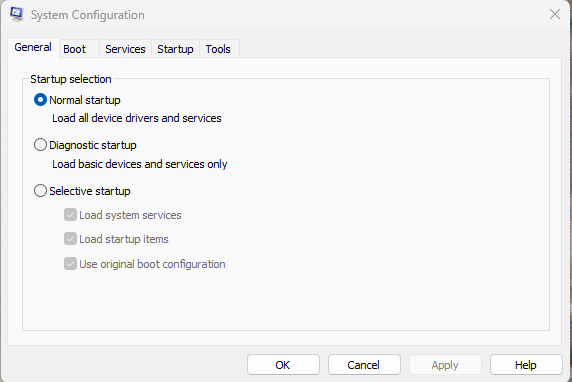
\includegraphics[width=0.99\linewidth]{sysconfig.png}%
}
\end{minipage}

